%Inserir Figura
%observação: as figuras estão sendo feitas no GeoGebra, aplicativo online para a criação de figuras

\documentclass[a4paper, 12pt]{article}
\usepackage[top=2cm, bottom=2cm, left=2.5cm, right=2.5cm]{geometry}
\usepackage[utf8]{inputenc}
\usepackage{amsmath, amsfonts, amssymb} 
\usepackage{graphicx} %pacote para a inserção de figuras
\usepackage{float} %pacote para inserir figuras no local certinho que a pessoa quer que a figura seja colocada
\usepackage[portuguese]{babel} %na referência de uma figura, colocá-la em português ("Figura 1" em vez de "Figure 1", por exemplo)


\begin{document}

\begin{enumerate}
    \item Calcule o valor de $x$ na Figura \ref{meu-outro-teste-rotulo}: %referenciar uma figura com rótulo
    
    \begin{figure}[htb] %função para a inserção da imagem.
                        %htb nos diz a prioridade do local onde a figura irá ser colocada. h = here, t = top, b = bottom. Assim, primeiro, o LaTeX tentará colocar a figura no local especificado. Caso não consiga, ele irá colocar no topo do documento. Por fim, caso ele não consiga colocar no topo, ele irá colocar embaixo do documento
                        
    
    %\begin{figure}[H]%com o pacote \usepackage{float}, pode-se substituir "htb" por "H". Neste caso, não tem jeito. A imagem irá ficar certinha no local em que você quer que ela fique
    
        \centering %centraliza a imagem 
        
        \includegraphics[scale=1]{exercicio.png} %o comando inclui a imagem ao documento. scale muda o tamanho da imagem que você quer que apareça. Não esqueça. Ampliar uma imagem pequena apresenta um resultado pior do que vocẽ fazer uma imagem grande e diminuir seu tamanho
        
        \caption{Questão sobre triângulo} %coloca a legenda da figura
        
        \label{meu-outro-teste-rotulo} %criar uma referência de figura para ser utilizada no texto
    \end{figure}
    
     \item Calcule o valor de $x$ na Figura \ref{meu-rotulo}:
    
    \begin{figure}[H]
        \centering
        \includegraphics[scale=1]{imagens/exercicio.png} %colocar imagens localizada em uma pasta
        \caption{Questão sobre triângulo} 
        \label{meu-rotulo} 
    \end{figure}

\end{enumerate}

\end{document}